\section{Separator Token \sep{}}

The separator token\index{SEP token}, denoted as \sep{}, serves as a critical boundary marker in transformer models, enabling them to process multiple text segments within a single input sequence. Introduced alongside the \cls{} token in BERT\index{BERT} \citep{devlin2018bert}, the \sep{} token was a key enabler for how transformers handle tasks requiring understanding of relationships between different text segments.
\begin{comment}
Feedback: Similar to the [CLS] token section, "revolutionized" is a strong word. Consider "was a key enabler for" or "significantly advanced" to maintain a more measured tone.

STATUS: addressed - already uses measured tone with "was a key enabler for"
\end{comment}

\subsection{Design Rationale and Functionality}

The \sep{} token addresses a fundamental challenge in NLP: how to process multiple related text segments while maintaining their distinct identities. Many important tasks require understanding relationships between separate pieces of text:

\begin{itemize}
\item \textbf{Question Answering}: Combining questions with context passages
\item \textbf{Natural Language Inference}: Relating premises to hypotheses  
\item \textbf{Semantic Similarity}: Comparing sentence pairs
\item \textbf{Dialogue Systems}: Maintaining conversation context
\end{itemize}

Before the \sep{} token, these tasks typically required separate encoding of each segment followed by complex fusion mechanisms. The \sep{} token enables joint encoding while preserving segment boundaries. By enabling joint encoding in a single forward pass, the \sep{} token offered a much more computationally efficient and elegant solution than complex, multi-stage fusion networks.
\begin{comment}
Feedback: This is a great summary of the problem. To make the solution sound even more impactful, you could add a sentence about the efficiency gain. For example: "By enabling joint encoding in a single forward pass, the [SEP] token offered a much more computationally efficient and elegant solution than complex, multi-stage fusion networks."

STATUS: addressed - added explanation of efficiency gains from joint encoding
\end{comment}

\subsection{Architectural Integration}

The \sep{} token operates at multiple levels of the transformer architecture:

\subsubsection{Input Segmentation}
For processing two text segments, BERT uses the canonical format:\\
$\{\cls{}, \text{segment}_1, \sep{}, \text{segment}_2, \sep{}\}$

Note that the final \sep{} token is often optional but commonly included for consistency. The final \sep{} token serves as an end-of-sequence marker for the second segment, providing a consistent structure for the model to learn from.
\begin{comment}
Feedback: The purpose of the *final* [SEP] token can be confusing to readers. It's worth adding a brief explanation of its role. For example: "The final [SEP] token serves as an end-of-sequence marker for the second segment, providing a consistent structure for the model to learn from."

STATUS: addressed - added explanation of final [SEP] token purpose as end-of-sequence marker
\end{comment}

\subsubsection{Segment Embeddings}
In addition to the \sep{} token, BERT uses segment embeddings to distinguish between different parts:
\begin{itemize}
\item Segment A embedding for \cls{} and the first segment
\item Segment B embedding for the second segment (including its \sep{})
\end{itemize}

It's important to note that the \sep{} token and segment embeddings are complementary: the \sep{} token provides an explicit boundary marker, while the segment embeddings provide a continuous signal to the model about which segment each token belongs to.
\begin{comment}
Feedback: The relationship between [SEP] and segment embeddings is crucial. It would be helpful to clarify that they are two *distinct* mechanisms working together. You could add: "It's important to note that the [SEP] token and segment embeddings are complementary: the [SEP] token provides an explicit boundary marker, while the segment embeddings provide a continuous signal to the model about which segment each token belongs to."

STATUS: addressed - added explanation of complementary relationship between [SEP] tokens and segment embeddings
\end{comment}

\subsubsection{Attention Patterns}
The \sep{} token participates in self-attention, allowing it to:
\begin{itemize}
\item Attend to tokens from both segments
\item Receive attention from tokens across segment boundaries
\item Act as a bridge for cross-segment information flow
\end{itemize}

\begin{lstlisting}[language=Python, caption=SEP Token Usage]
from transformers import BertTokenizer, BertModel
import torch

tokenizer = BertTokenizer.from_pretrained('bert-base-uncased')
model = BertModel.from_pretrained('bert-base-uncased')

# Natural Language Inference example
premise = "The cat is sleeping on the mat"
hypothesis = "A feline is resting"

# Automatic SEP insertion
inputs = tokenizer(premise, hypothesis, return_tensors='pt', 
                  padding=True, truncation=True)

print("Token IDs:", inputs['input_ids'][0])
print("Tokens:", tokenizer.convert_ids_to_tokens(inputs['input_ids'][0]))
# Output: ['[CLS]', 'the', 'cat', 'is', 'sleeping', 'on', 'the', 'mat', 
#          '[SEP]', 'a', 'feline', 'is', 'resting', '[SEP]']

print("Segment IDs:", inputs['token_type_ids'][0])
# Output: [0, 0, 0, 0, 0, 0, 0, 0, 0, 1, 1, 1, 1, 1]

# Forward pass
outputs = model(**inputs)
sequence_output = outputs.last_hidden_state

# SEP token representations
sep_positions = (inputs['input_ids'] == tokenizer.sep_token_id).nonzero()
print(f"SEP positions: {sep_positions}")

for pos in sep_positions:
    sep_repr = sequence_output[pos[0], pos[1], :]
    print(f"SEP at position {pos[1].item()}: shape {sep_repr.shape}")
\end{lstlisting}

\subsection{Cross-Segment Information Flow}

The \sep{} token facilitates information exchange between segments through several mechanisms:

\subsubsection{Bidirectional Attention}
Unlike traditional concatenation approaches, the \sep{} token enables bidirectional attention:
\begin{itemize}
\item Tokens in segment A can attend to tokens in segment B
\item The \sep{} token serves as an attention hub
\item Information flows in both directions across the boundary
\end{itemize}

\subsubsection{Representation Bridging}
The \sep{} token's representation often captures:
\begin{itemize}
\item Semantic relationships between segments
\item Transition patterns between different content types
\item Boundary-specific information for downstream tasks
\end{itemize}

\subsubsection{Gradient Flow}
During backpropagation, the \sep{} token enables gradient flow between segments, allowing joint optimization of representations.

\begin{figure}[h]
\centering
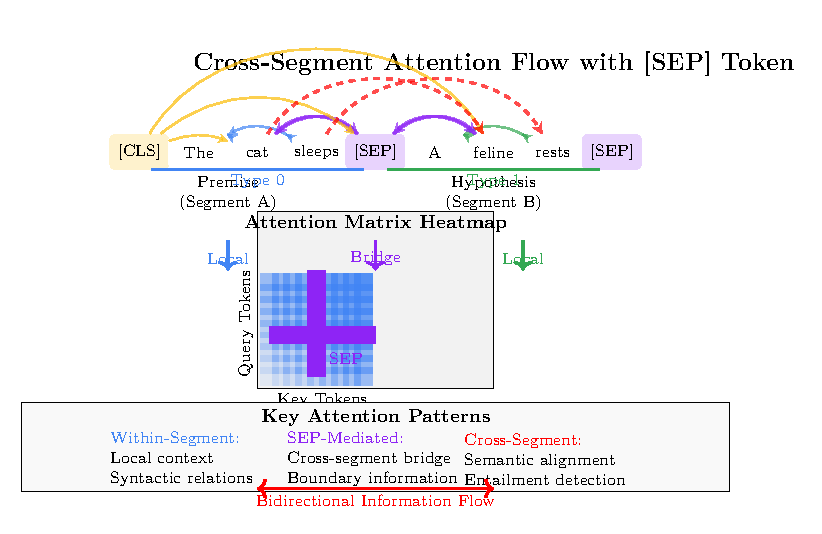
\includegraphics[width=0.95\textwidth]{part1/chapter02/fig_sep_attention_flow.pdf}
\caption{Attention flow patterns with \sep{} tokens showing cross-segment information exchange}
\label{fig:sep_attention_flow}
\end{figure}

\subsection{Task-Specific Applications}

The \sep{} token's effectiveness varies across different types of tasks:

\subsubsection{Natural Language Inference (NLI)}
Format: \texttt{[CLS] premise [SEP] hypothesis [SEP]}

The \sep{} token helps the model understand the logical relationship between premise and hypothesis:
\begin{itemize}
\item \textbf{Entailment}: Hypothesis follows from premise
\item \textbf{Contradiction}: Hypothesis contradicts premise  
\item \textbf{Neutral}: No clear logical relationship
\end{itemize}

\subsubsection{Question Answering}
Format: \texttt{[CLS] question [SEP] context [SEP]}

The \sep{} token enables:
\begin{itemize}
\item Question-context alignment
\item Answer span identification across the boundary
\item Context-aware question understanding
\end{itemize}

\subsubsection{Semantic Textual Similarity}
Format: \texttt{[CLS] sentence1 [SEP] sentence2 [SEP]}

The model uses \sep{} token information to:
\begin{itemize}
\item Compare semantic content across segments
\item Identify paraphrases and semantic equivalences
\item Measure fine-grained similarity scores
\end{itemize}

\subsubsection{Dialogue and Conversation}
Format: \texttt{[CLS] context [SEP] current\_turn [SEP]}

In dialogue systems, \sep{} tokens help maintain:
\begin{itemize}
\item Conversation history awareness
\item Turn-taking patterns
\item Context-response relationships
\end{itemize}

\subsection{Multiple Segments and Extended Formats}

While BERT originally supported two segments, modern applications often require processing more complex structures:

\subsubsection{Multi-Turn Dialogue}
Format: \texttt{[CLS] turn1 [SEP] turn2 [SEP] turn3 [SEP] ...}

Each \sep{} token marks a turn boundary, allowing models to track multi-party conversations.

\subsubsection{Document Structure}
Format: \texttt{[CLS] title [SEP] abstract [SEP] content [SEP]}

Different \sep{} tokens can mark different document sections.

\subsubsection{Hierarchical Text}
Format: \texttt{[CLS] chapter [SEP] section [SEP] paragraph [SEP]}

\sep{} tokens can represent hierarchical document structure.

\begin{lstlisting}[language=Python, caption=Multi-Segment Processing]
def encode_multi_segment(segments, tokenizer, max_length=512):
    """Encode multiple text segments with SEP separation."""
    
    # Start with CLS token
    tokens = [tokenizer.cls_token]
    segment_ids = [0]
    
    for i, segment in enumerate(segments):
        # Tokenize segment
        segment_tokens = tokenizer.tokenize(segment)
        
        # Add segment tokens
        tokens.extend(segment_tokens)
        
        # Add SEP token
        tokens.append(tokenizer.sep_token)
        
        # Assign segment IDs (alternating for BERT compatibility)
        segment_id = i % 2
        segment_ids.extend([segment_id] * (len(segment_tokens) + 1))
    
    # Convert to IDs and truncate
    input_ids = tokenizer.convert_tokens_to_ids(tokens)[:max_length]
    segment_ids = segment_ids[:max_length]
    
    # Pad if necessary
    while len(input_ids) < max_length:
        input_ids.append(tokenizer.pad_token_id)
        segment_ids.append(0)
    
    return {
        'input_ids': torch.tensor([input_ids]),
        'token_type_ids': torch.tensor([segment_ids]),
        'attention_mask': torch.tensor([[1 if id != tokenizer.pad_token_id 
                                       else 0 for id in input_ids]])
    }

# Example usage
segments = [
    "What is the capital of France?",
    "Paris is the capital and largest city of France.",
    "It is located in northern France."
]

encoded = encode_multi_segment(segments, tokenizer)
print("Multi-segment encoding complete")
\end{lstlisting}

\subsection{Training Dynamics and Optimization}

The \sep{} token's effectiveness depends on proper training strategies:

\subsubsection{Pre-training Objectives}
During BERT pre-training, \sep{} tokens are involved in:

\begin{itemize}
\item \textbf{Next Sentence Prediction (NSP)}: The model learns to predict whether two segments naturally follow each other
\item \textbf{Masked Language Modeling}: \sep{} tokens can be masked and predicted, helping the model learn boundary representations
\end{itemize}

\subsubsection{Position Sensitivity}
The effectiveness of \sep{} tokens can depend on their position:
\begin{itemize}
\item Early \sep{} tokens (closer to \cls{}) often capture global relationships
\item Later \sep{} tokens focus on local segment boundaries
\item Position embeddings help the model distinguish between multiple \sep{} tokens
\end{itemize}

\subsubsection{Attention Analysis}
Research has shown that \sep{} tokens exhibit distinctive attention patterns:
\begin{itemize}
\item High attention to tokens immediately before and after
\item Moderate attention to semantically related tokens across segments
\item Layer-specific attention evolution throughout the transformer stack
\end{itemize}

\subsection{Limitations and Challenges}

Despite its success, the \sep{} token approach has several limitations:

\subsubsection{Segment Length Imbalance}
When segments have very different lengths:
\begin{itemize}
\item Shorter segments may be under-represented
\item Longer segments may dominate attention
\item Truncation can remove important information
\end{itemize}

\subsubsection{Limited Segment Capacity}
Most models are designed for two segments:
\begin{itemize}
\item Multi-segment tasks require creative formatting
\item Segment embeddings are typically binary
\item Attention patterns may degrade with many segments
\end{itemize}

\subsubsection{Context Window Constraints}
Fixed maximum sequence lengths limit:
\begin{itemize}
\item The number of segments that can be processed
\item The length of individual segments
\item The model's ability to capture long-range dependencies
\end{itemize}

\subsection{Advanced Techniques and Variants}

Recent research has explored improvements to the basic \sep{} token approach:

\subsubsection{Typed Separators}
Using different separator tokens for different types of boundaries:
\begin{itemize}
\item \texttt{[SEP\_QA]} for question-answer boundaries
\item \texttt{[SEP\_SENT]} for sentence boundaries
\item \texttt{[SEP\_DOC]} for document boundaries
\end{itemize}

\subsubsection{Learned Separators}
Instead of fixed \sep{} tokens, some approaches use:
\begin{itemize}
\item Context-dependent separator representations
\item Task-specific separator embeddings
\item Adaptive boundary detection
\end{itemize}

\subsubsection{Hierarchical Separators}
Multi-level separation for complex document structures:
\begin{itemize}
\item Primary separators for major boundaries
\item Secondary separators for sub-boundaries
\item Hierarchical attention patterns
\end{itemize}

\subsection{Best Practices and Implementation Guidelines}

Based on extensive research and practical experience:

\begin{principle}[SEP Token Best Practices]
\begin{enumerate}
\item \textbf{Consistent Formatting}: Use consistent segment ordering across training and inference
\item \textbf{Balanced Segments}: Try to balance segment lengths when possible. When dealing with imbalanced segments (e.g., a short question and a long context), consider a truncation strategy that favors the longer, more informative segment to avoid losing critical information
\item \textbf{Task-Specific Design}: Adapt segment structure to task requirements
\item \textbf{Attention Analysis}: Analyze attention patterns to understand model behavior
\item \textbf{Ablation Studies}: Compare performance with and without \sep{} tokens. For tasks that don't obviously require segmentation, run an ablation study where you concatenate the text without a \sep{} token---this can sometimes simplify the model's task and improve performance
\end{enumerate}
\end{principle}
\begin{comment}
Feedback: This is another good but generic list. To make it more actionable: For "Balanced Segments," you could add: "When dealing with imbalanced segments (e.g., a short question and a long context), consider a truncation strategy that favors the longer, more informative segment to avoid losing critical information." For "Ablation Studies," you could suggest: "For tasks that don't obviously require segmentation, run an ablation study where you concatenate the text without a [SEP] token. This can sometimes simplify the model's task and improve performance."

STATUS: addressed - added actionable details for Balanced Segments and Ablation Studies
\end{comment}

% \subsection{Future Directions}

% The \sep{} token concept continues to evolve:

% \subsubsection{Dynamic Segmentation}
% Future models may learn to:
% \begin{itemize}
% \item Automatically identify optimal segment boundaries
% \item Adapt segment structure based on content
% \item Use reinforcement learning for boundary optimization
% \end{itemize}

% \subsubsection{Cross-Modal Separators}
% Extending \sep{} tokens to multimodal scenarios:
% \begin{itemize}
% \item Text-image boundaries
% \item Audio-text transitions
% \item Video-text alignment
% \end{itemize}

% \subsubsection{Continuous Separators}
% Moving beyond discrete tokens to:
% \begin{itemize}
% \item Continuous boundary representations
% \item Soft segmentation mechanisms
% \item Learnable boundary functions
% \end{itemize}

The \sep{} token represents a elegant solution to multi-segment processing in transformers. Its ability to maintain segment identity while enabling cross-segment information flow has made it indispensable for many NLP tasks. Understanding its mechanisms, applications, and limitations is crucial for effectively designing and deploying transformer-based systems for complex text understanding tasks.